\byline{{\textbf{\Large\sffamily TWBC Workshops:}}\\
        {\textbf{\large\sffamily A Night of Insights with Peter Warren}}}{Nick Lloyd}
\label{2025-09-workshop}
\noindent
Our most recent club meeting saw a full house and an eager crowd, all gathered for a special critique session led by the ever\--knowledgeable Peter Warren.
After a warm introduction from the chairman Tony Ulatowski, the evening kicked off with a row of members' trees ready to face the spotlight\dots{} and Peter wasted no time getting stuck in.

\medskip
\topic{Tony's Hawthorn}
\noindent
Starting with Tony's Hawthorn, Peter guided us through his approach to critique: a process rooted in asking the right questions.
What species is it?
Is the tree healthy enough to work on?
If the answer to that last one is no, then the priority must always be restoring health before anything else.
From there, the conversation turned to identifying character features --- those unchangeable elements like nebari, trunk movement, mature bark or deadwood, and how they guide decisions on styling and choosing the best front.

It was fascinating to watch Peter break things down so methodically.
He highlighted how personal taste and emotional attachment play their part, but ultimately, every tree benefits from a consistent, thoughtful process.
Questions around balance, proportion, and branch development were common threads throughout the evening.
In the case of Tony's Hawthorn, Peter encouraged selective growth to improve proportion --- especially thickening up lower branches by letting them extend over time, while keeping the top in check.

\begin{window}[%
    2,l,%
    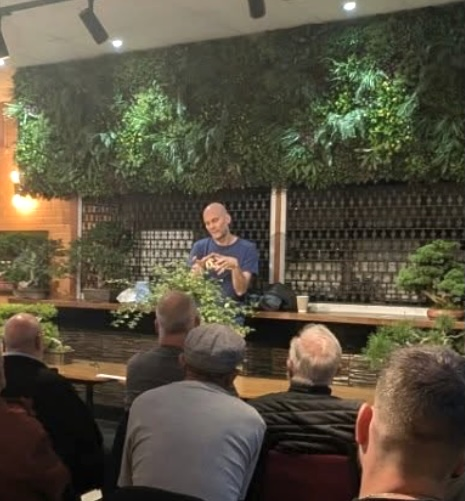
\includegraphics[width=1.0\columnwidth]{2025_09/res/workshop_peter},%
    \centerline{\emph{Peter offers expert feedback during our club's critique night.}}%
]
\end{window}
\columnbreak

\medskip
\topic{David's Scots Pine}
\noindent
Next up was David Kilvington's rather wild\--looking Scots pine, affectionately dubbed `The Octopus'.
Estimated to be around 50 years old, this tree presented a different challenge.
Peter pointed out that its current width and depth exceeded its height, throwing the visual balance off.
Some light trimming was done on the spot, removing dead and weak growth to tidy the image.
He also noted that on a tree of this age, the likelihood of back budding is low due to branch maturity --- meaning its structure is, for the most part, set.
The challenge now is working with what's already there.

\medskip
\topic{Grant's Beuvronensis Pine}
\noindent
Then came Grant Kinnaird's Scots pine `Beuvronensis' --- a younger tree, but with great promise.
Peter praised the variety's naturally smaller needle size, which lends itself well to bonsai.
Unlike David's older pine, this one has more developmental potential.
Peter explained how, with careful candle pinching and well\--timed pruning (typically around late July to August), back budding could be encouraged to help refine the tree's silhouette over time.

\medskip
\topic{The Three of Yews}
\noindent
We then looked at three Yews (Taxus baccata), each at different stages of development.
One belonged to the club, and the others to Mark Edwards and Brendan Gibbs.
The club tree could benefit from a repotting into a larger container with better drainage --- a simple fix with big impact.
Brendan's tree, meanwhile, was in recovery after a run\--in with vine weevils.
A valuable reminder here: vine weevils love fleshy roots (as in yews and tridents) and dislike bonsai soils with larger particle sizes.
Peter recommended treating future infestations with nematodes --- a natural and effective approach.

\medskip
\topic{Juniper Snares}
\noindent
The final set included three very different junipers: a garden variety brought by Terry Wilson, a Kishu owned by Chris Hallewell, and a recently purchased Itoigawa from Chris Durne.
Terry's tree, which had a notably coarse `male' foliage due to flowering, might be a Sabina juniper --- a bit of a mystery, but full of character.
The Kishu and Itoigawa junipers were both fine examples of their kind, with Peter offering advice on refining branch placement and structure to enhance their form further.

\medskip
\topic{Final Words}
\noindent
Throughout the evening, Peter's calm and considered approach reminded us all that good bonsai comes from thoughtful questioning and careful planning --- not rushed decisions.
His practical advice was backed by years of experience, but always delivered with encouragement and a touch of humour that kept the atmosphere warm and engaging.

Huge thanks again to Peter for sharing his insight with us, and to all who came along and made the evening such a success.
Whether you brought a tree or just came to listen, there was something for everyone to take away.
\closearticle
\clearpage

\end{multicols}

\begin{center}
    \begin{minipage}[b]{.43\textwidth}
        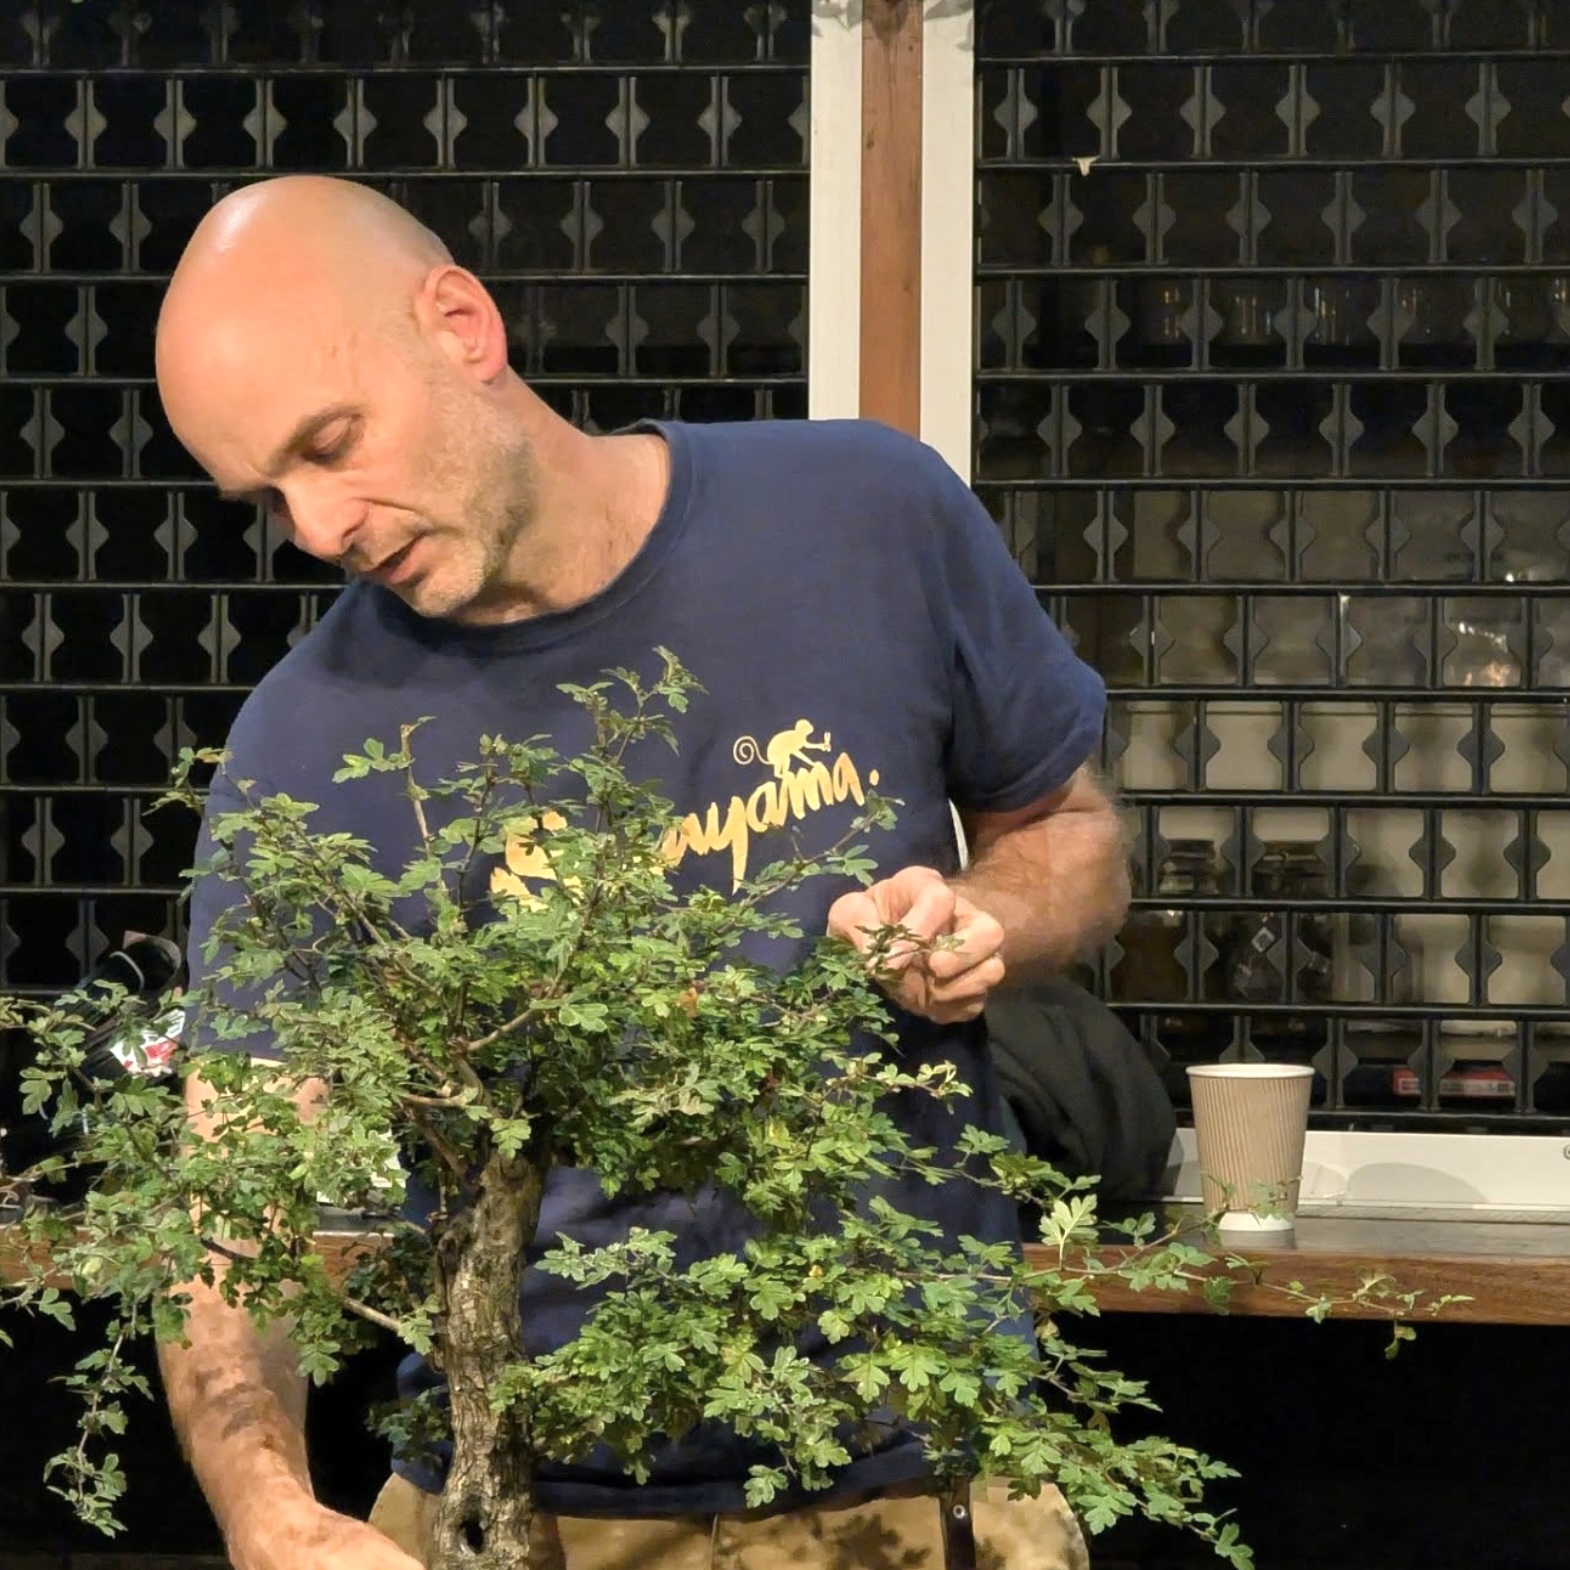
\includegraphics[angle=0,origin=c,width=1.0\textwidth]{2025_09/res/workshop_warren3.jpg}
    \end{minipage}\quad
    \begin{minipage}[b]{.43\textwidth}
        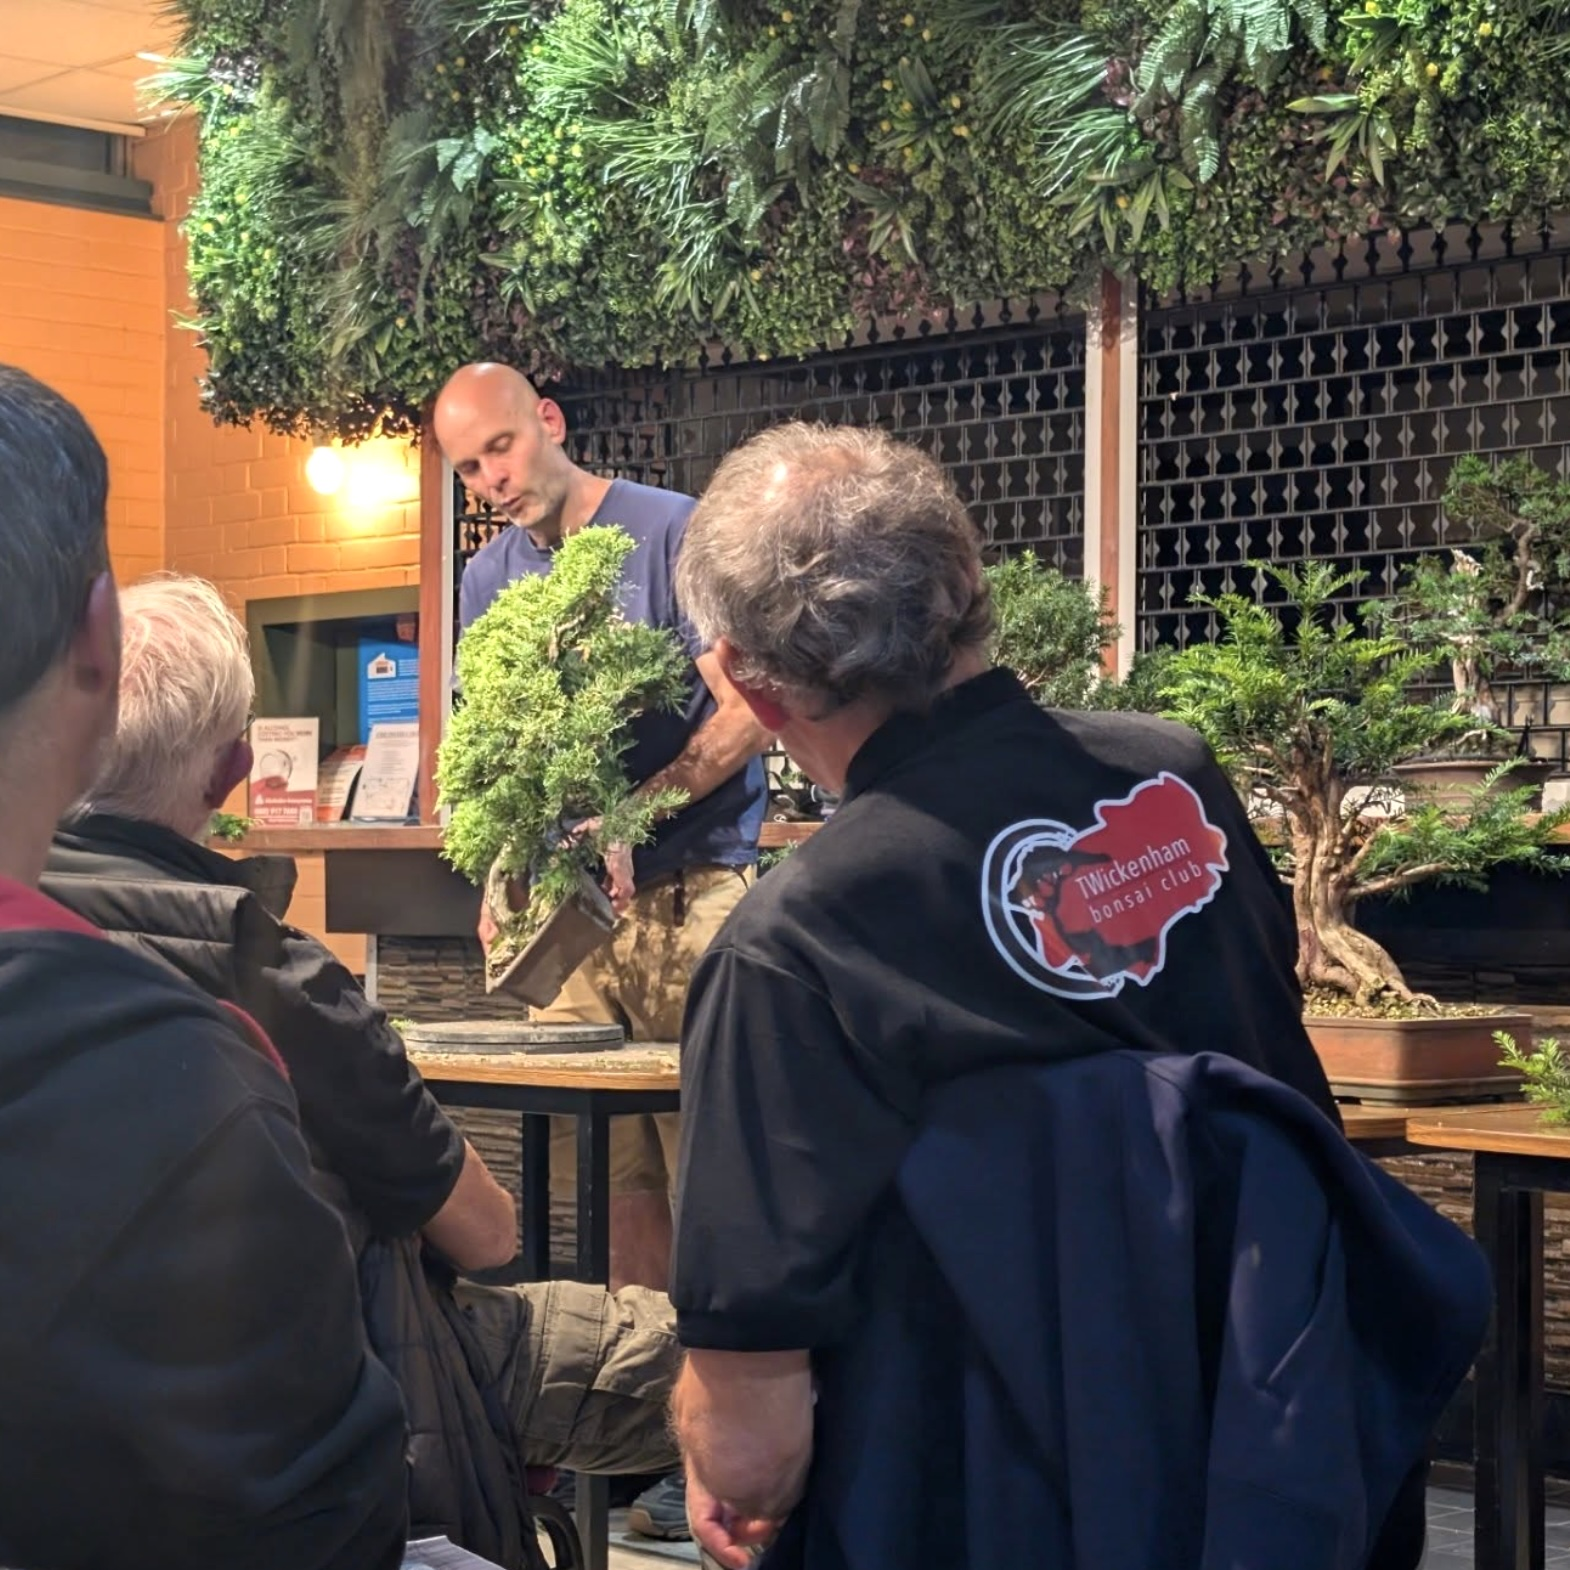
\includegraphics[angle=0,origin=c,width=1.0\textwidth]{2025_09/res/workshop_warren1.jpg}
    \end{minipage}
    \medskip

    \begin{minipage}[b]{.43\textwidth}
        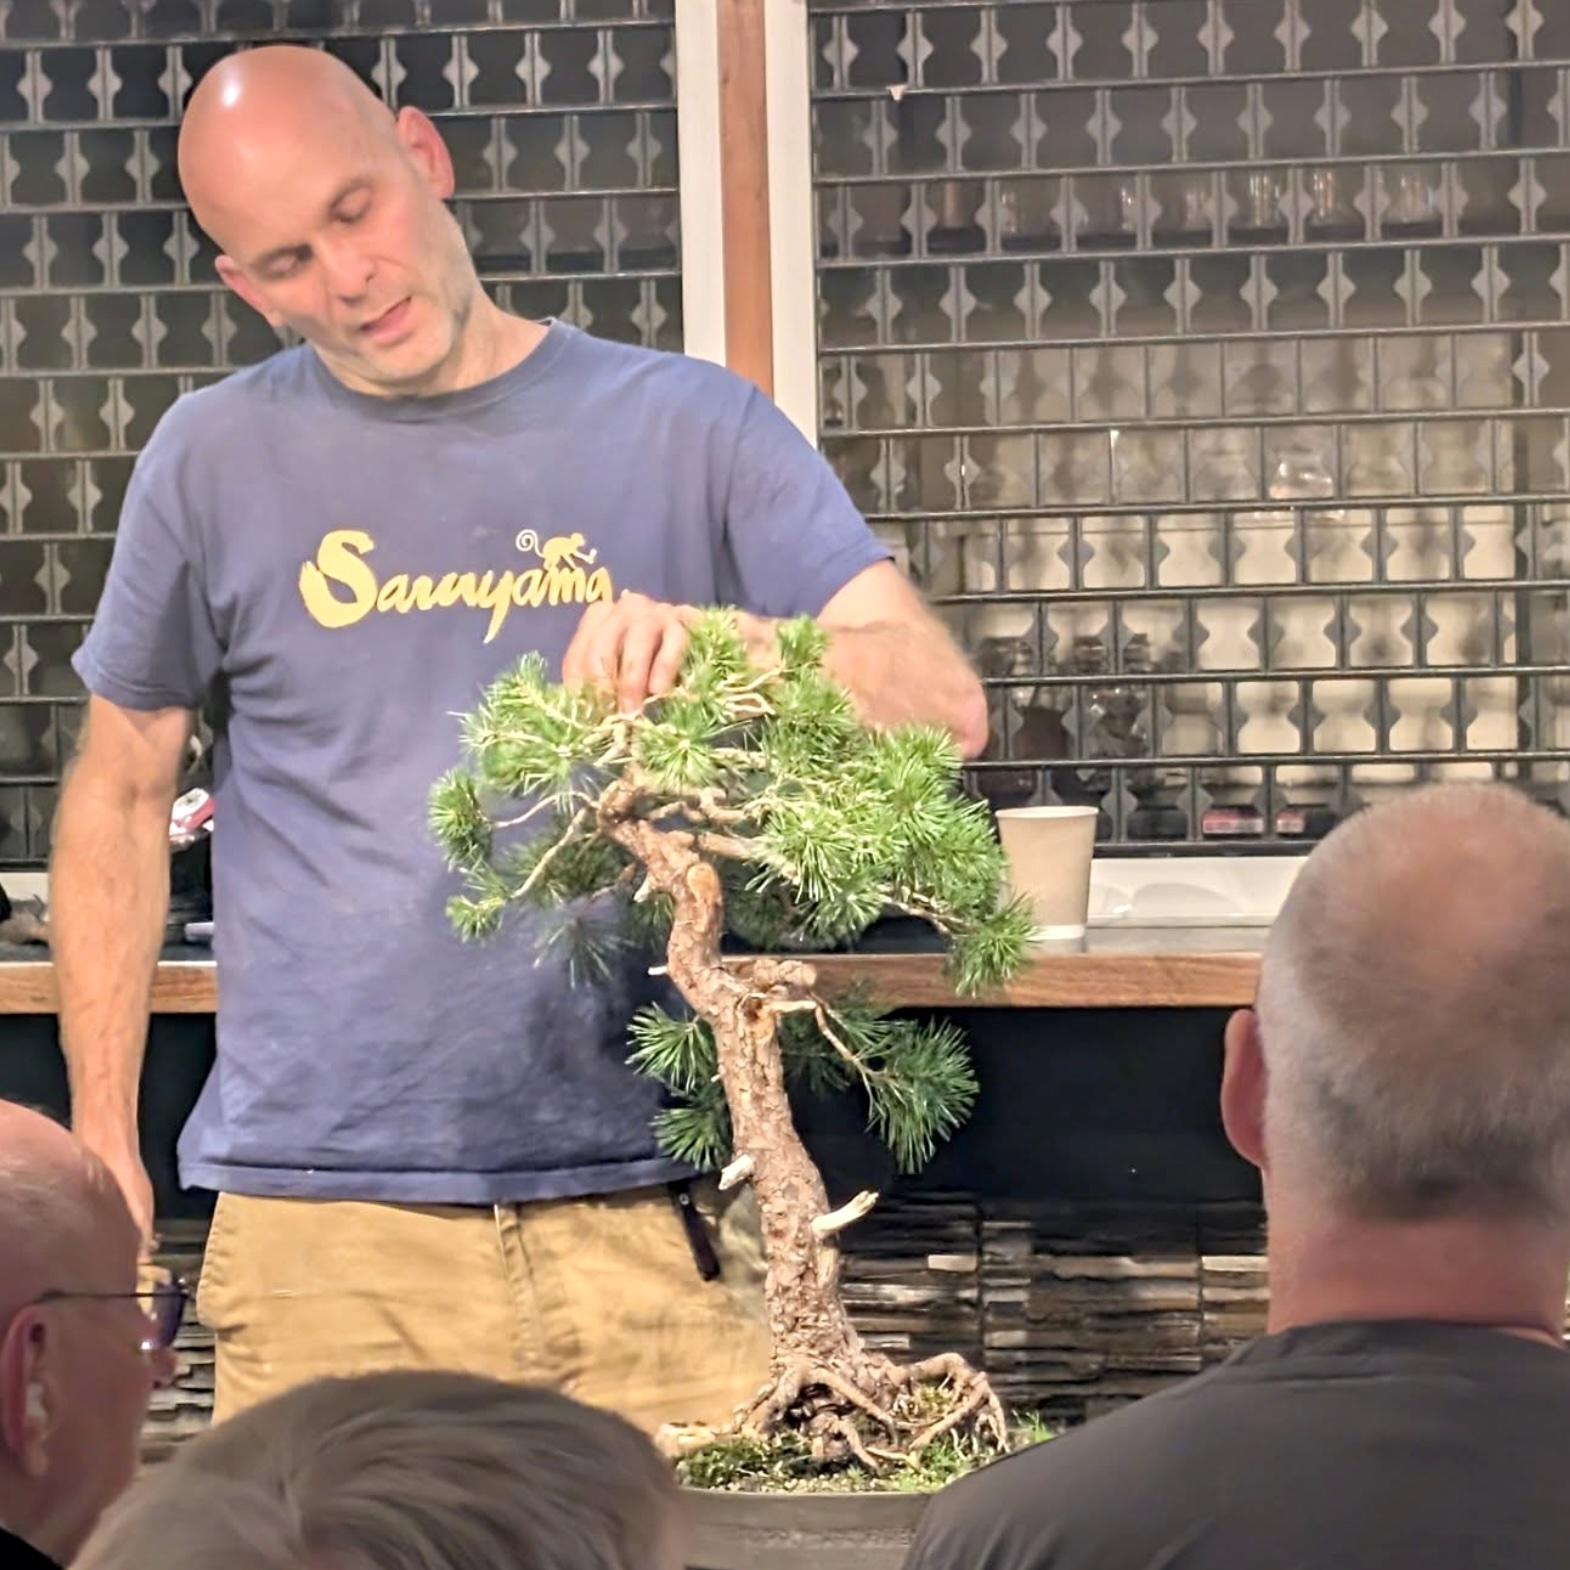
\includegraphics[angle=0,origin=c,width=1.0\textwidth]{2025_09/res/workshop_warren5.jpg}
    \end{minipage}\quad
    \begin{minipage}[b]{.43\textwidth}
        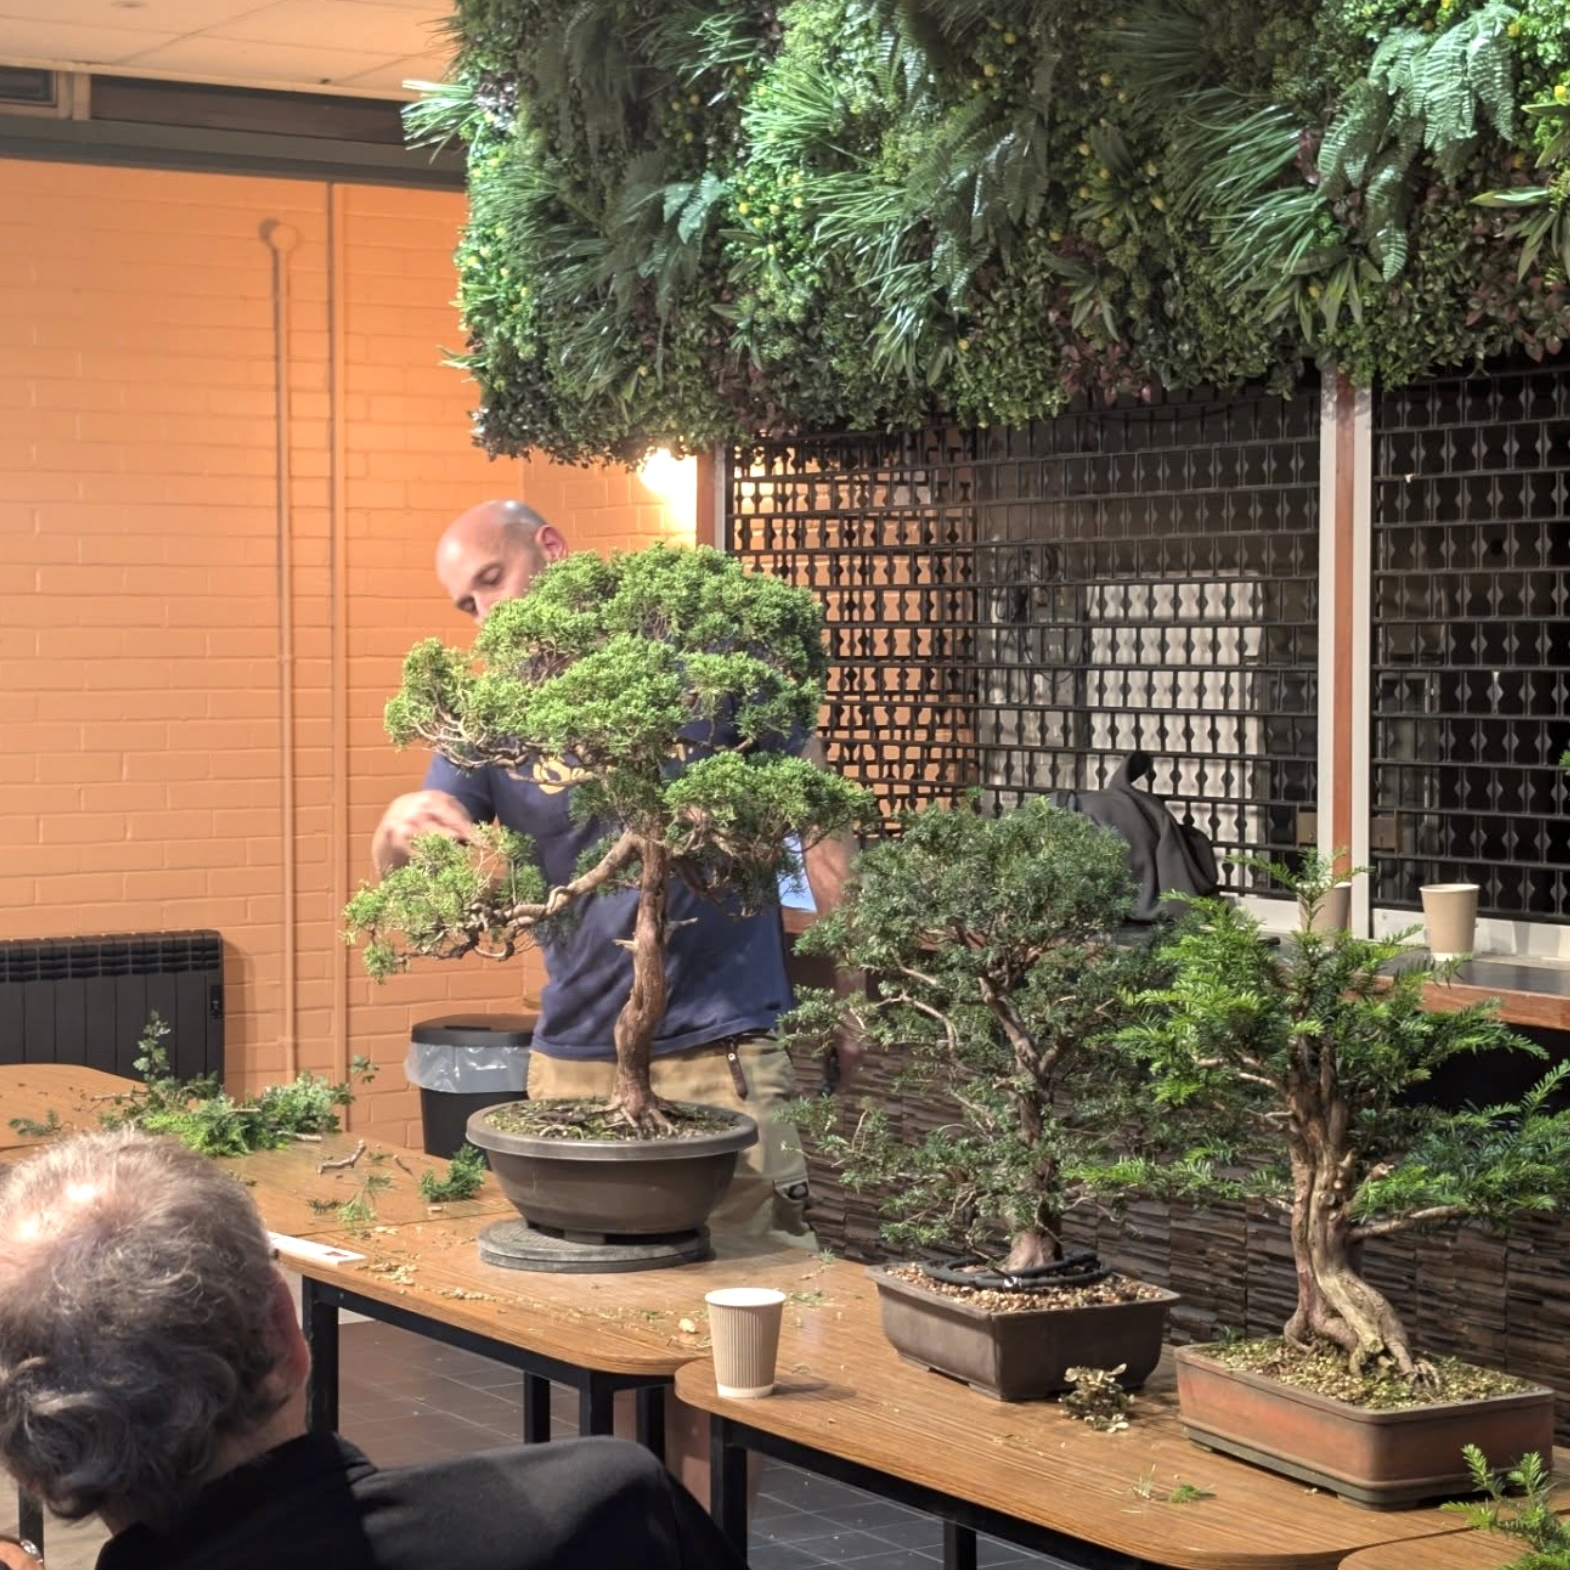
\includegraphics[angle=0,origin=c,width=1.0\textwidth]{2025_09/res/workshop_warren2.jpg}
    \end{minipage}
    \medskip

    \begin{minipage}[b]{.43\textwidth}
        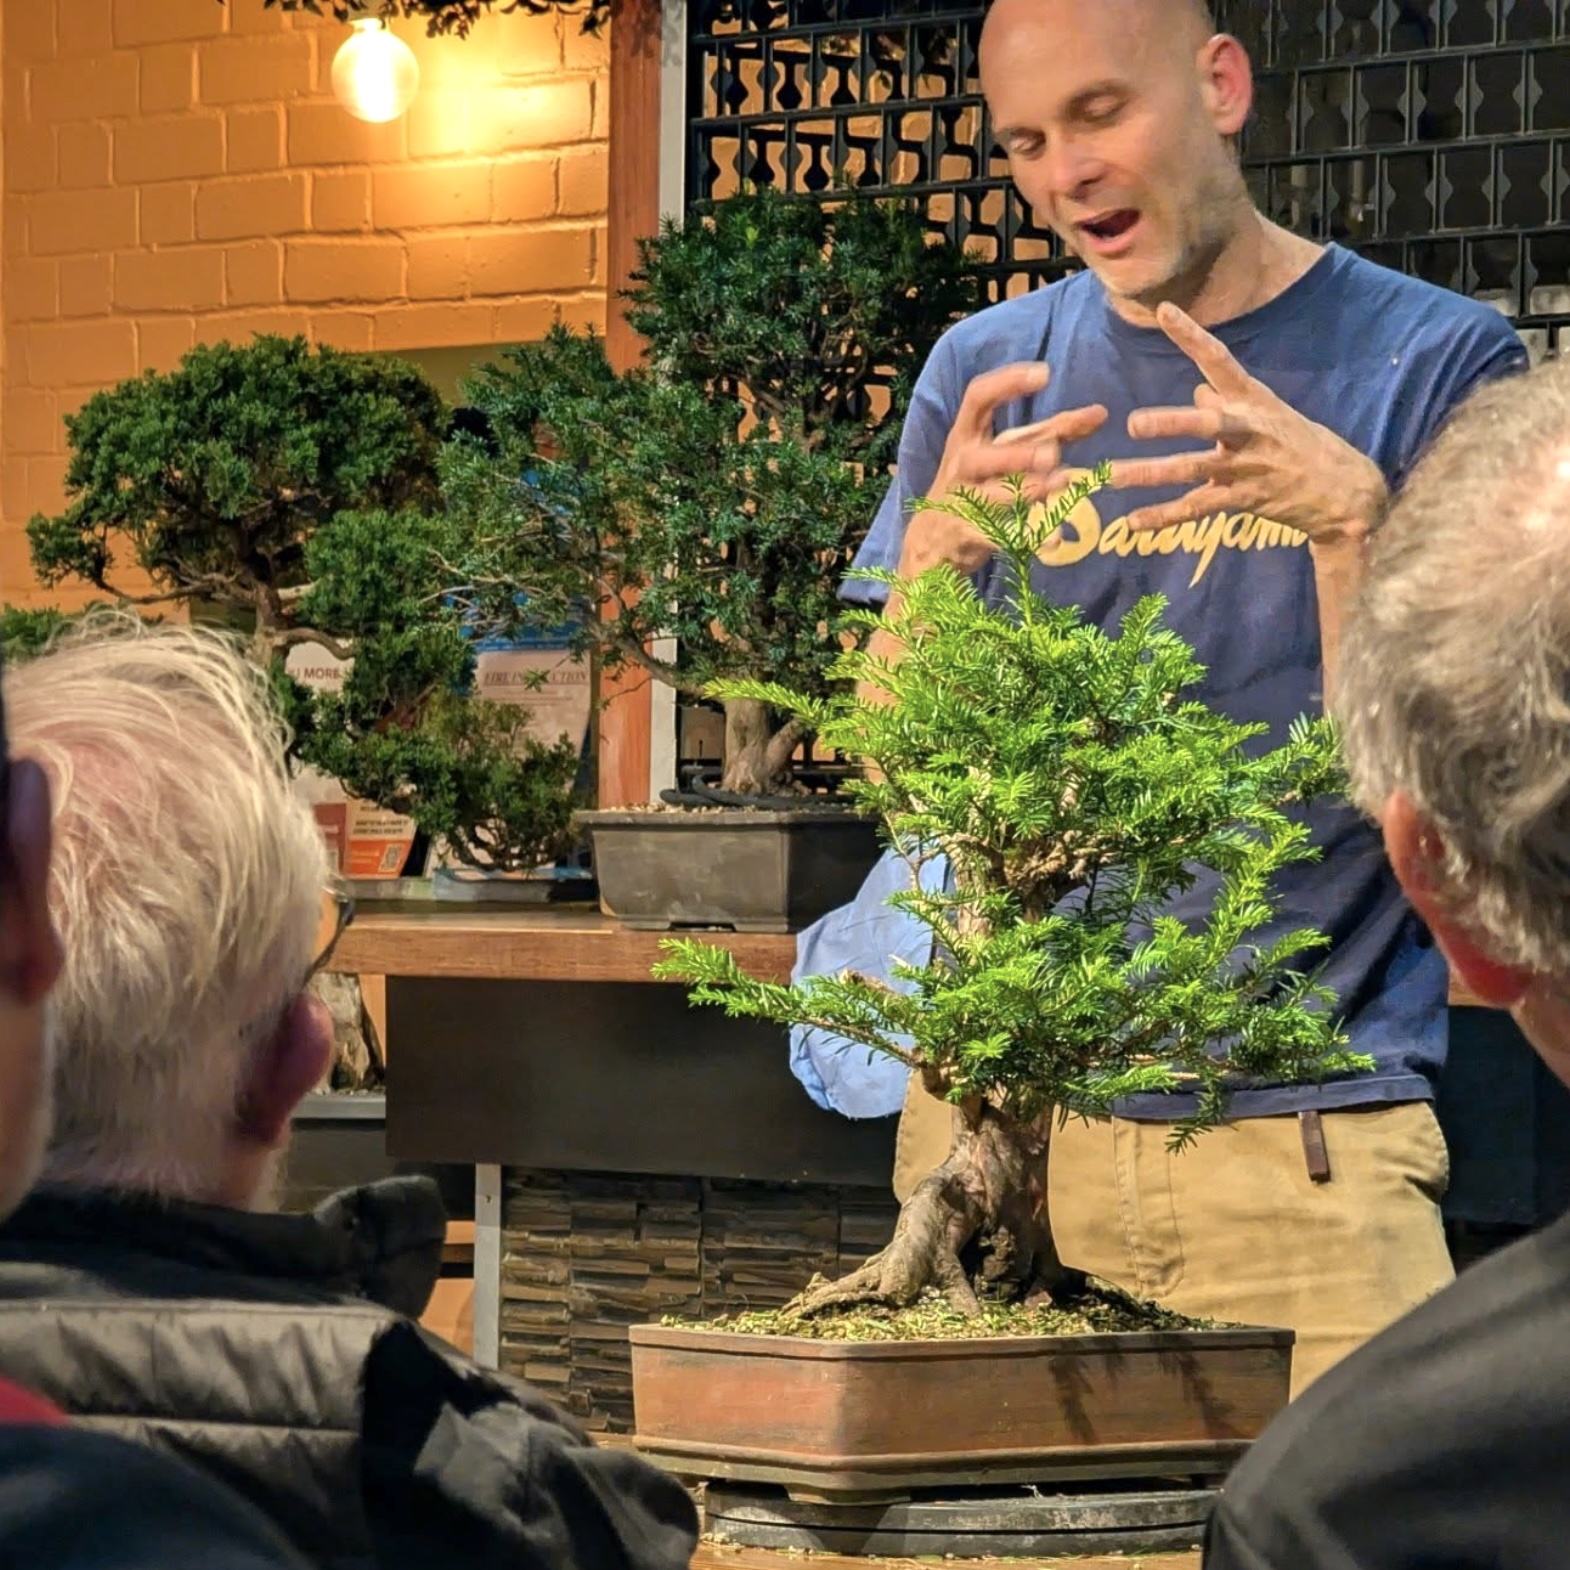
\includegraphics[angle=0,origin=c,width=1.0\textwidth]{2025_09/res/workshop_warren6.jpg}
    \end{minipage}\quad
    \begin{minipage}[b]{.43\textwidth}
        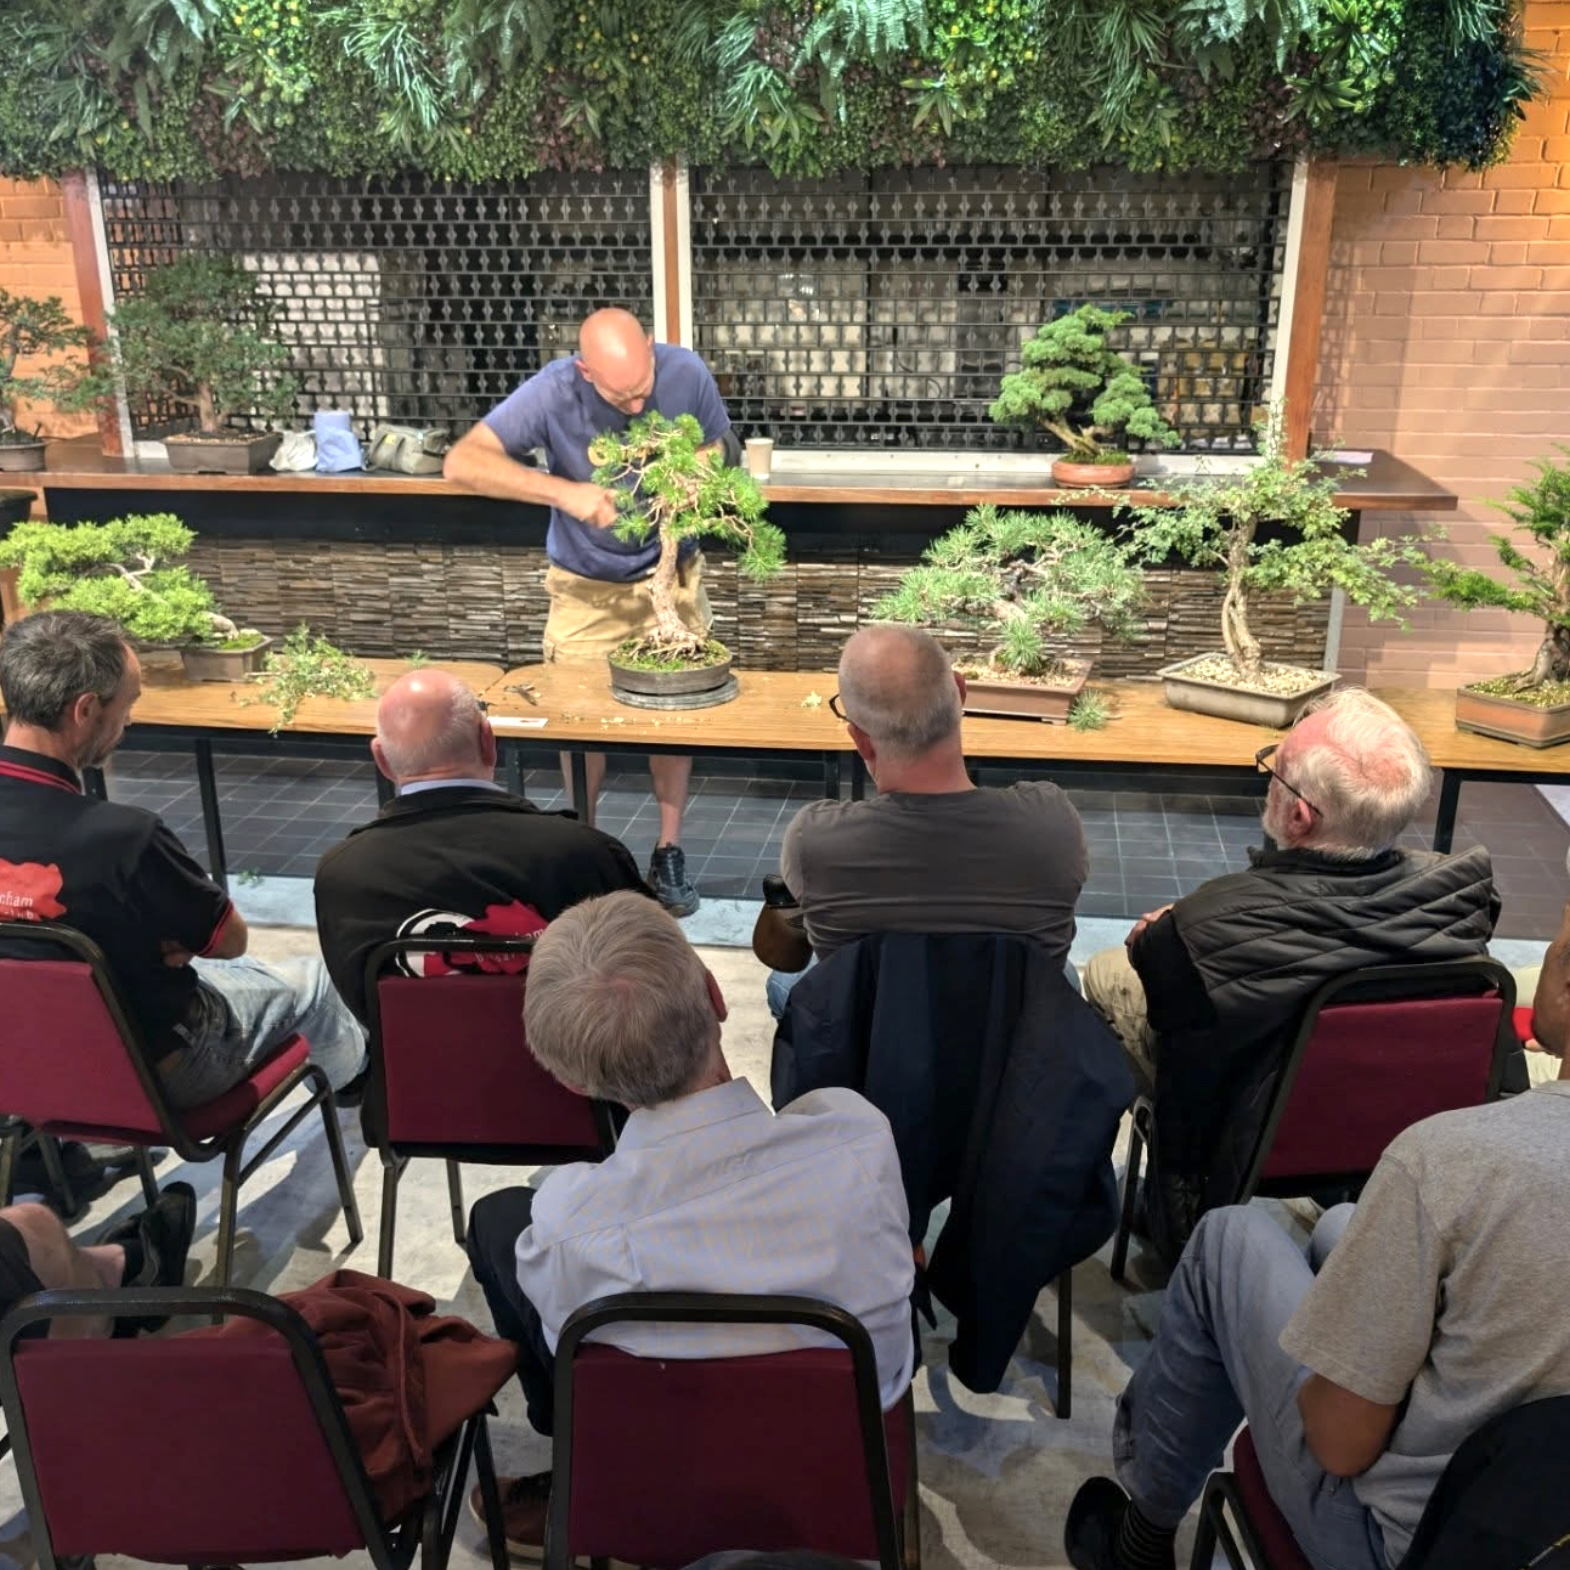
\includegraphics[angle=0,origin=c,width=1.0\textwidth]{2025_09/res/workshop_warren4.jpg}
    \end{minipage}
    \medskip

    \emph{A few highlights from the critique night with Peter Warren during last club meeting.}
\end{center}

\begin{multicols}{2}
\clearpage
